%======================================================================
%----------------------------------------------------------------------
%               XX                           X
%                                            X
%               XX    XXX   XXX   XXX   XXX  X  XXXX
%                X   X   X X   X X   X X   X X X
%                X   XXXXX XXXXX XXXXX X     X  XXX
%                X   X     X     X     X   X X     X
%               XXX   XXX   XXX   XXX   XXX  X XXXX
%----------------------------------------------------------------------
%  	         SPECIFICATION FOR COMMON IEEE STYLES
%----------------------------------------------------------------------
%               Gregory L. Plett, Istv\'{a}n Koll\'{a}r.
%======================================================================
\documentclass[%
	%draft,
	%submission,
	%compressed,
	final,
	%
	%technote,
	%internal,
	%submitted,
	%inpress,
	reprint,
	%
	%titlepage,
	notitlepage,
	%anonymous,
	narroweqnarray,
	inline,
	twoside,
        invited,
	]{ieee}

\newcommand{\latexiie}{\LaTeX2{\Large$_\varepsilon$}}
%\usepackage{ieeetsp}	% if you want the "trans. sig. pro." style
%\usepackage{ieeetc}	% if you want the "trans. comp." style
%\usepackage{ieeeimtc}	% if you want the IMTC conference style

% Use the `endfloat' package to move figures and tables to the end
% of the paper. Useful for `submission' mode.
%\usepackage {endfloat}

% Use the `times' package to use Helvetica and Times-Roman fonts
% instead of the standard Computer Modern fonts. Useful for the 
% IEEE Computer Society transactions.
%\usepackage{times}
% (Note: If you have the commercial package `mathtime,' (from 
% y&y (http://www.yandy.com), it is much better, but the `times' 
% package works too). So, if you have it...
%\usepackage {mathtime}

% for any plug-in code... insert it here. For example, the CDC style...
%\usepackage{ieeecdc}

\begin{document}

%----------------------------------------------------------------------
% Title Information, Abstract and Keywords
%----------------------------------------------------------------------
\title[Sistema de reproducción de mp3 usando GStreamer y Qt]{%
       Sistema de reproducción de mp3 usando GStreamer y Qt}

% format author this way for journal articles.
% MAKE SURE THERE ARE NO SPACES BEFORE A \member OR \authorinfo
% COMMAND (this also means `don't break the line before these
% commands).
\author[PLETT AND KOLL\'{A}R]{Luis Carrillo, Sergio Gonzales, Angel Phillips \authorinfo{e-mail: glp@simoon.stanford.edu}%
\and{}and Istv\'{a}n Koll\'{a}r\member{Fellow}\authorinfo{I.\
       Koll\'{a}r is with the Department of Measurement and Information
       Systems, Technical University of Budapest, 1521 Budapest, Hungary.
       Phone: $+$\,36\,1\,463--1774, fax: +\,36\,1\,463--4112, 
       e-mail: kollar@mmt.bme.hu}
}

% format author this way for conference proceedings
%\author[PLETT AND KOLL\'{A}R]{%
        %Gregory L. Plett\member{Student Member},\authorinfo{%
        %Department of Electrical Engineering,\\ 
        %Stanford University, Stanford, CA 94305-9510.\\
        %Phone: $+$1\,650\,723-4769, email: glp@simoon.stanford.edu}%
%\and{}and%
%\and{}Istv\'{a}n Koll\'{a}r\member{Fellow}\authorinfo{%
        %Department of Measurement and Instrument Engineering,\\ 
        %Technical University of Budapest, 1521 Budapest, Hungary.\\
        %Phone: $+$\,36\,1\,463-1774, fax: +\,36\,1\,463-4112, 
        %email: kollar@mmt.bme.hu}
%}
\journal{IEEE Trans.\ on Instrum.\ Meas.}
\titletext{, VOL.\ 46, NO.\ 6, DECEMBER\ 1997}
\ieeecopyright{0018--9456/97\$10.00 \copyright\ 1997 IEEE}
\lognumber{xxxxxxx}
\pubitemident{S 0018--9456(97)09426--6}
\loginfo{Manuscript received September 27, 1997.}
\firstpage{1}

\confplacedate{Ottawa, Canada, May 19--21, 1997}

\maketitle               

\begin{abstract} 
 En este documento se describe, de manera general, el proceso de diseo e implementacin del sistema de reproduccin de mp3, la idea esta implementacin fue la desarrollar una aplicacin basada en la plataforma multimedia Gstreamer , la cual fuera sintetizable en una plataforma embebidos como Beaglebord-xM, adems que permitiera la interaccin con otros dispositivos mediantes redes de comunicacin.
\end{abstract}

\begin{keywords}
Beagleboard-xM, GStreamer, Qt Creator
\end{keywords}

%----------------------------------------------------------------------
% SECTION I: Introduction
%----------------------------------------------------------------------
\section{Introduction}

\PARstart El objetivo de este proyecto es desarrollar un sistema de reproduccin de archivos de audio en formato mp3, empleando GStreamer y Qt Creator en una Beagleboard-xM.

Los principales objetivos de diseo de la aplicacin son:

\begin{itemize}
\item Desarrollar una aplicacin para la Beagleboard-xM, la cual se utilizar como dispositivo maestro, en la que se pueda seleccionar y reproducir un archivo mp3.
\item Se debe poder reproducir de manera local o enviar un stream de audio para ser reproducido en una PC remota. 
\item Desarrollar una aplicacin para PC, la cual permite reproducir el stream que recibe de la Beagleboard.
\end{itemize}

Una de las herramientas principales del proyecto, es la famosa Beagleboard-xM (hardware libre). La gran ventaja de este tipo de placas es que es son lo suficientemente potentes en cuanto a memoria y velocidad de procesamiento para permitir la instalacin de un OS y acceder al control del hardware a travs de l. Este empotrado cuenta con un procesador DM3730 basado en un ncleo ARM Cortex-A8, frecuencia de trabajo de 1 GHz. Capacidad de video en HD (Texas Instruments C64x + Procesador DSP), tambin tiene 512 MB de memoria RAM DDR, puertos de comunicacin: I2C, I2S, SPI, 4 puertos Host USB, 1 puerto serie RS-232, 1 JTAG para depuracion y una conexion 10/100 Ethernet. Tiene un seal de audio estreo de entrada y salida para altavoces y micrfono, salida de video: DVI-D y S-video, conector de expansin para LCD, conector para cmara digital y para fuente de alimentacin externa de 5V cc y un slot para tarjetas de memoria micro-SD, como se muestra en la siguiente figura:

\begin{figure}[hbtp]
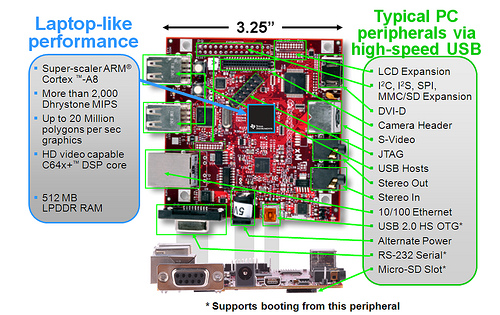
\includegraphics[scale=0.5]{beagleboard.jpg}
\caption{Beagleboard-mX}
\end{figure}


Se utiliza GStreamer ya que es una biblioteca la cual permite el manejo de componentes multimedia, por es posible desarrollar aplicaciones que reproduzcan video, audio, utilicen cmaras, entre otras. Esta biblioteca basa su funcionamiento en complementos lo cuales proveen ms funcionalidades y codecs para reproducir diferentes tipos de archivos.

Los elementos de Gstreamer consisten en sources, filtros y sinks. Un grupo de elementos tambin es llamado un bin. El bin de mayor nivel es llamado pipeline. El pipeline puede ser controlado para  cambiar el estado a reproducir, pausar etc. Otro concepto usado frecuentemente son los pads. Los elementos poseen source pads y sink pads. Un pipeline conecta un flujo desde los source pads hasta los sink pads  y con esto logra reproducir archivos, hacer streaming, entre otros.
%----------------------------------------------------------------------
% SECTION II: The Document Life-Cycle
%----------------------------------------------------------------------
\section{Descripcin del diseño e implementación del sistema}

En primera instancia, lo  primero que se hizo fue tratar de entender el problema que se nos pide resolver. Se nos pide hacer una aplicacion que corra en la beagleboard (como servidor), con una interfaz grfica que le permita al usuario donde quiere reproducir la cancin deseada, ya sea en su propio servidor (beagleboard) o en una computadora remota, como se visualiza en la figura siguiente:

\begin{figure}[hbtp]
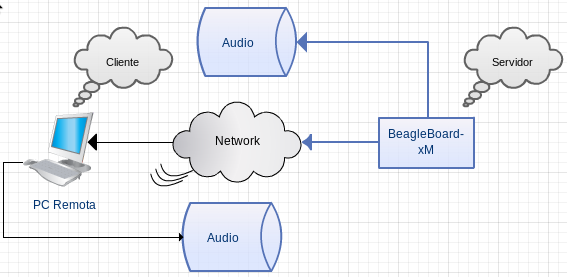
\includegraphics[scale=0.5]{Diagrama1.png}
\caption{Esquema cliente-servidor}
\end{figure}

Para desarrollar las aplicaciones primero se investig gstreamer y sus capacidades de reproduccin y streaming, se buscaron y probaron pipelines que cumplieran con los requerimientos, como por ejemplo:

Servidor:

\begin{figure}[hbtp]
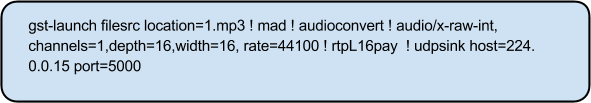
\includegraphics[scale=0.4]{sHLG4TD6qldYM4Yfh1m1DlA.png}
\caption{Pipeline UDP Server}
\end{figure}

Cliente:

\begin{figure}[hbtp]
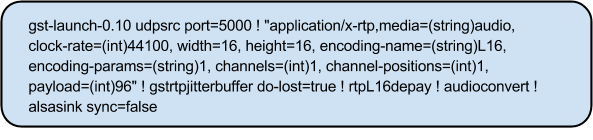
\includegraphics[scale=0.4]{sq5lrprsXxVFWBa8R1s-7yg.png}
\caption{Pipeline UDP Client}
\end{figure}

Estos pipelines se probaron en la beagleboard para ver si era necesario instalar bibliotecas en esta.
Luego de encontrar el pipeline, se empez la investigacin de como pasarlo al lenguaje C, para as poder construir la aplicacin en Qt. Cuando se logra traducir el pipeline a C se une el código, junto con la GUI para as tener la funcionalidad completa.

%----------------------------------------------------------------------
% SECTION III: Specifications
%----------------------------------------------------------------------
\section{Implementación}

Se procedió a realizar el desarrollo de las interfaces gráficas tanto de servidor con el cliente en la plataforma de programación QtCreator, en la fig. se muestra el diseño final de la interfaz del servidor, esta contiene botones de reproducción (play), detección(stop), pausa y de cargar de archivo mp3, además se agregó una lista de reproducción que permite al usuario agregar varios archivo mp3, también se tienen espacios de texto para agregar las direcciones ip, ya que al ser el servidor debe enviar la información al cliente.

\begin{figure}[hbtp]
\includegraphics[scale=0.3]{servidor.png}
\caption{Interfaz Servidor}
\end{figure}



%----------------------------------------------------------------------
% SECTION VII: Conclusions
%----------------------------------------------------------------------
\section{Conclusion}

\begin{itemize}
\item La beagleboard-xM es un embebido muy poderoso, capaz de resolver problemas con un grado de dificultad bastante elevado y de forma muy eficiente.
\item Qt Creator permite realizar interfaces gráficas muy amigables con el usuario, y a la vez opaca la dificultad de programar en C.
\item ¿A que un reproductor de audio parecía algo complejo? En realidad no lo es tanto. En una era como la actual, en la que el vídeo y el audio han tomado todo, es muy sencillo integrarlos en nuestra aplicación. Podemos, incluso, añadir tutoriales en vídeo a nuestro programa. Y sólo hemos rozado la superficie, GStreamer posee un API muy completo de manipulación de flujos multimedia, y gracias a los plugin está siempre al día. Quizá sea esa la razón por la cual después de tanto tiempo sigue estando en la versión 0.10; el desarrollo se ha desplazado del núcleo a los plugins. Sea como fuere, GStreamer se integra perfectamente con C.
\end{itemize}

%----------------------------------------------------------------------
% The bibliography. This bibliography was generated using the following
% two lines:
%\bibliographystyle{IEEEbib}
%\bibliography{ieeecls}
% where, the contents of the ieeecls.bib file was:
%
%@book{lamport,
%        AUTHOR = "Leslie Lamport",
%         TITLE = "A Document Preparation System: {\LaTeX} User's Guide
%                  and Reference Manual",
%       EDITION = "Second",
%     PUBLISHER = "Addison-Wesley",
%       ADDRESS = "Reading, MA",
%          YEAR = 1994,
%          NOTE = "Be sure to get the updated version for \LaTeX2e!"
%}
%
%@book{goossens,
%        AUTHOR = "Michel Goossens and Frank Mittelbach and
%                  Alexander Samarin",
%         TITLE = "The {\LaTeX} Companion",
%     PUBLISHER = "Addison-Wesley",
%       ADDRESS = "Reading, MA",
%          YEAR = 1994,
%}
%
% The ieeecls.bbl file was manually included here to make the distribution
% of this paper easier. You need not do it for your own papers.

\begin{thebibliography}{1}

\bibitem{lamport}
http://beagleboard.org/Products/BeagleBoard-xM

\bibitem{goossens}
http://gstreamer.freedesktop.org/

\end{thebibliography}

%----------------------------------------------------------------------
\end{document}
